\documentclass[9pt,twocolumn]{report}
%%%%%%%%%%%%%%%%%%%%%%%%%%%Definition
%%%%%%%%%%%%%%%%%%%%%to who
\newcommand{\Client}{Delin Li}
\newcommand{\ClientF}{Li}
\newcommand{\Inst}{NGS Center}
\newcommand{\Email}{delin.bio@gmail.com}

\newcommand{\Company}{XXX Center} %DGC
\newcommand{\SeqPlatform}{Illumina} %DGC

%species and reference genome
\newcommand{\Species}{Maize}
\newcommand{\Specieslatin}{\textit{Zea mays}}
\newcommand{\SampleNumber}{188}
\newcommand{\Website}{JGI Phytozome v12 website}           %genome downloaded from
\newcommand{\WebsiteURL}{http://www.youtube.com/watch?v=tOV47_ogPWY}
\newcommand{\BaseSelection}{2}
\newcommand{\ReferenceGenome}{AGVRV2}
\newcommand{\ProjectPurpose}{construct a genetic map}
  
\newcommand{\Prefix}{Maize} %%%% file name prefix(species) no . or _ was allowed
 % will define the variable 
\title{Template for DL's Project}
\author{\clientfont \Client}
\affil{\sffamily\bfseries\LARGE Report Date: \dashdate\today}
\affil{\intfont  \Inst | E-mail: \Email}
%\correspondingauthor{\ClientF} %Family name of client 
\begin{abstract}
Here, the summary will be described with necessary information. Like total sample number:  \SampleNumber, NGS plateform  \SeqPlatform, the reference genome the \Specieslatin\ \ReferenceGenome\ reference genome.
\end{abstract}

\begin{document}
\maketitle
\thispagestyle{firststyle}
\logomark
\firstpagefootnote
\vspace{-20pt}
\vspace{-11pt}

\section{Workflow}
The background information: who \Client provided   \SampleNumber\ \Species\ samples for what purpose:\ \ProjectPurpose\.
And the analysis workflow: Figure \ref{workflow}. \par

\begin{figure}[ht]
\centering
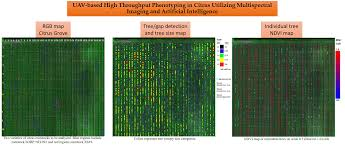
\includegraphics[width=0.45\textwidth]{drone.jpeg}
\caption{A generalized workflow}
\label{workflow}
\end{figure} 

%\input{ReferenceGenome} % The reference genome information could be summaried here.

 
%%%%%%%%%%%%%%%%%%%%
%%%%%%%Section I
%%%%%%%%%%%%%%%%%%%%

\section{Section Summary I}
Necessary information for the first section I with table and/or figure\ref{NGS:SectI}.\\
%\input{NGS_reads} This is a table 

\begin{figure}[!ht]
\centering
\scriptsize
    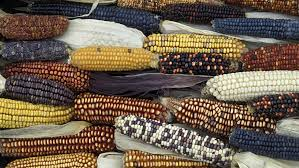
\includegraphics[width=0.48\textwidth]{maize.jpeg}
\caption{Maize}
\label{NGS:SectI}
\end{figure}

%%%%%%%%%%%%%%%%%%%%
%%%%%%%Section II 
%%%%%%%%%%%%%%%%%%%%
\section{Section Summary II}

\subsection{Subsection}
\paragraph{Give detail Criteria like SNPs filtering:}
\begin{itemize}
		\item Requre how many or percentage samples covered.
		\item The MAF $\leqslant$1\%
		\item The Heter
\end{itemize}	

%%%%%%%%%%%%%%%%%%%%
%%%%%%%Section III
%%%%%%%%%%%%%%%%%%%%
\section{Section Summary III}
Summary in section III with tables and/or figure \ref{wheat:fig}.


\begin{figure}[ht]
\centering
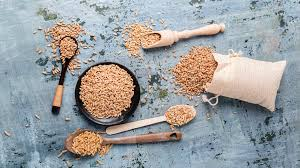
\includegraphics[width=0.48\textwidth]{wheat.jpeg} %{\Prefix_MCR50_snps_genotype_summary_by_sample.pdf}
\caption{Caption: Wheat}
\label{wheat:fig}
\end{figure}

%%%%%%%%%%%%%%%%%%%%
%%%%%%%Section IV
%%%%%%%%%%%%%%%%%%%%
\section{Section Summary IV}
Summary in section IV with tables and/or figure.% \ref{soy:fig}.
\iffalse 
\begin{figure}[htbp]
\renewcommand{\familydefault}{\sfdefault}\normalfont
\centering
\scriptsize
    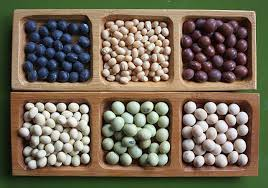
\includegraphics[width=0.45\textwidth]{soybean.jpeg} %{\Prefix_missing_rate.pdf}
\caption{Caption: Soybean}
\label{soy:fig}
\end{figure}
\fi

%%%%%%%%%%%%%%%%%%%%
%%%%%%% Section V
%%%%%%%%%%%%%%%%%%%%
\section{Outputs}
Give a list of files will deliver.
\begin{itemize}
%\begin{enumerate}
\renewcommand{\labelenumi}{\alph{enumi}}
		\item \textbf{\seqsplit{\Prefix.vcf}}: The genotype in vcf format.
		\item \textbf{\seqsplit{\Prefix.geneticmap.txt}}: The constructed genetic map.
% \end{enumerate}
\end{itemize}


%%%%%%%%%%%%%%%%%%%%
%%%%%%%Methods%BETA
%%%%%%%%%%%%%%%%%%%%
\section{Methods}
Give the methods and citations.

\bibliographystyle{unsrtnat}%{plainnat}
\bibliography{report}

\end{document}
